% ---------------------------------------------------------------------------
% Drop-in figure environments for the TOMM manuscript (acmart, acmsmall).
% Copy the PDFs into the Overleaf project (e.g. figures/contrib/) and adjust
% the path. Every figure is drawn at \textwidth (13.9 cm), so text inside the
% figures stays at 6-7.5 pt after inclusion. acmart requires \Description.
% Preamble additions: \usepackage{tabularx}  (for the two tables)
% ---------------------------------------------------------------------------

\begin{figure}[t]
  \centering
  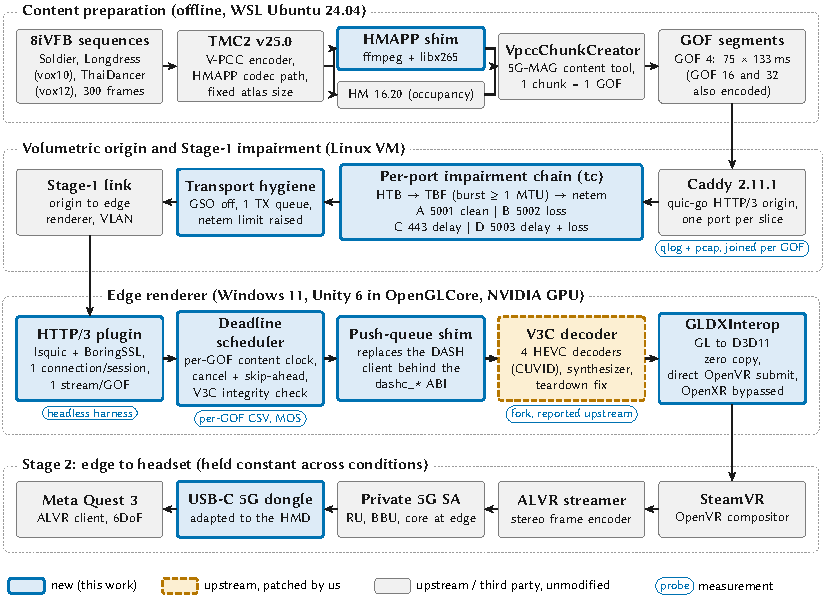
\includegraphics[width=\textwidth]{figures/contrib/fig1_overview.pdf}
  \caption{\textsc{MOSAIC} with the provenance of every component. Blue boxes are new, the dashed box is an upstream component we patched, grey boxes are used unmodified. Badges mark where measurements are taken.}
  \Description{Block diagram in four lanes. Content preparation: 8iVFB sequences, TMC2, an HMAPP shim to ffmpeg and libx265 next to HM for occupancy, the 5G-MAG chunker, and per-GOF segments. Origin: Caddy, a per-port tc impairment chain, transport hygiene, and the Stage-1 link. Edge renderer: HTTP/3 plugin, deadline scheduler, push-queue shim, patched V3C decoder, and GLDXInterop. Stage 2: SteamVR, ALVR, private 5G, an adapted USB-C 5G dongle, and the Meta Quest 3.}
  \label{fig:contrib-overview}
\end{figure}

\begin{figure}[t]
  \centering
  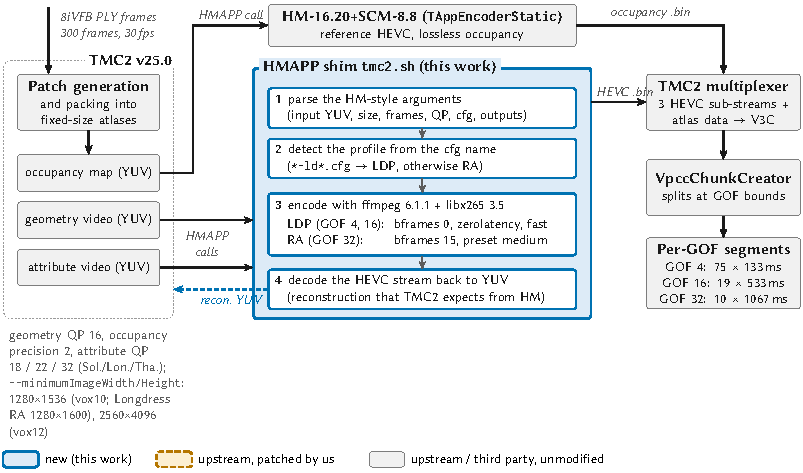
\includegraphics[width=\textwidth]{figures/contrib/fig2_encoder_shim.pdf}
  \caption{Encoder back end. TMC2 calls an external HM-style encoder per video sub-stream. Our shim answers the geometry and attribute calls with ffmpeg and libx265 and returns the reconstruction TMC2 expects, while the lossless occupancy map stays on HM.}
  \Description{TMC2 produces occupancy, geometry and attribute videos. Occupancy goes to HM. Geometry and attribute go to the shim, which parses HM arguments, detects the LDP or RA profile from the configuration name, encodes with ffmpeg 6.1.1 and libx265 3.5, and decodes the result back to YUV for TMC2. The multiplexer builds the V3C bitstream and the chunker splits it into per-GOF segments.}
  \label{fig:contrib-encoder}
\end{figure}

\begin{figure}[t]
  \centering
  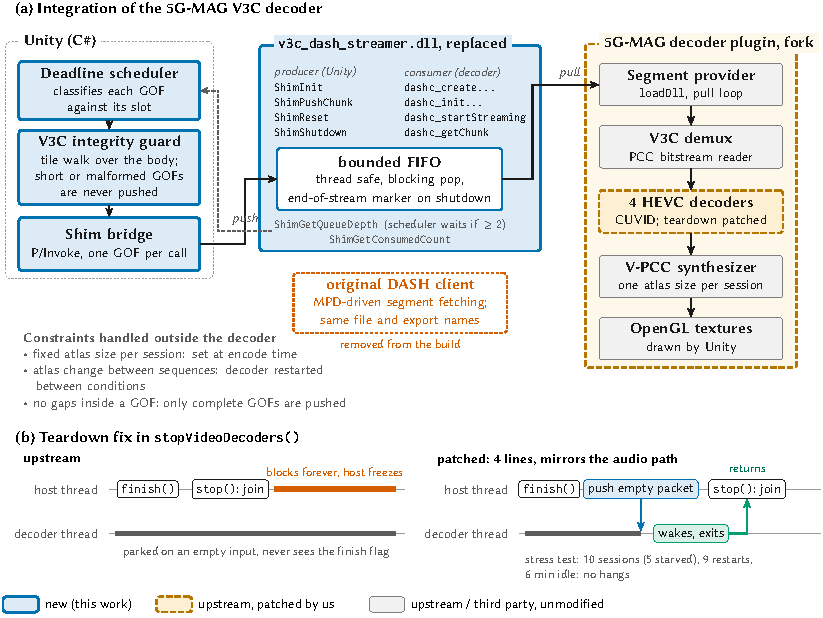
\includegraphics[width=\textwidth]{figures/contrib/fig3_decoder_integration.pdf}
  \caption{(a) The 5G-MAG decoder is fed through a replacement of its DASH client DLL that keeps the same exports and exposes a bounded FIFO to Unity. (b) The teardown fix: an empty packet wakes each parked video decoder thread before the join.}
  \Description{Panel a: Unity components (scheduler, integrity guard, shim bridge) push GOFs into a FIFO inside the replacement DLL; the decoder pulls through the dashc functions into demux, four HEVC decoders, the synthesizer and OpenGL textures. Panel b: two timelines. Upstream, the host thread blocks forever in join while the decoder thread waits on an empty input. Patched, the host pushes an empty packet, the decoder thread wakes and exits, and join returns.}
  \label{fig:contrib-decoder}
\end{figure}

\begin{figure}[t]
  \centering
  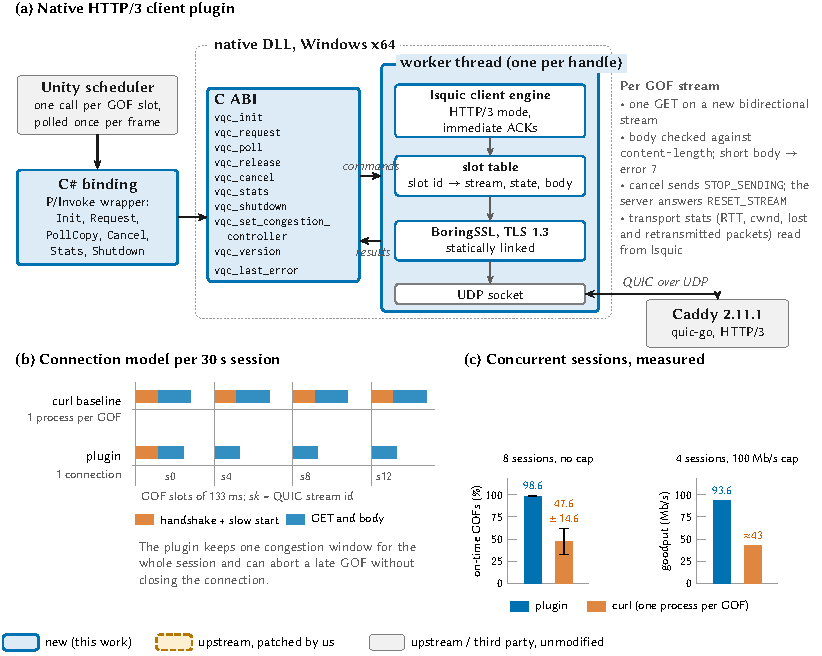
\includegraphics[width=\textwidth]{figures/contrib/fig4_http3_plugin.pdf}
  \caption{(a) Native HTTP/3 plugin built on lsquic. (b) One connection per session replaces one process and one handshake per GOF. (c) Measured with concurrent sessions at look-ahead 4 (error bar: standard deviation across runs).}
  \Description{Panel a: Unity calls a C\# binding, which calls a C ABI of ten functions; a worker thread holds the lsquic engine, a slot table, BoringSSL and a UDP socket toward Caddy. Panel b: timelines where curl repeats handshake and slow start for each GOF while the plugin performs one handshake and opens one stream per GOF. Panel c: bar charts, on-time GOFs 98.6 percent for the plugin and 47.6 percent for curl with eight sessions, and goodput 93.6 versus about 43 Mb/s with four sessions under a 100 Mb/s cap.}
  \label{fig:contrib-plugin}
\end{figure}

\begin{figure}[t]
  \centering
  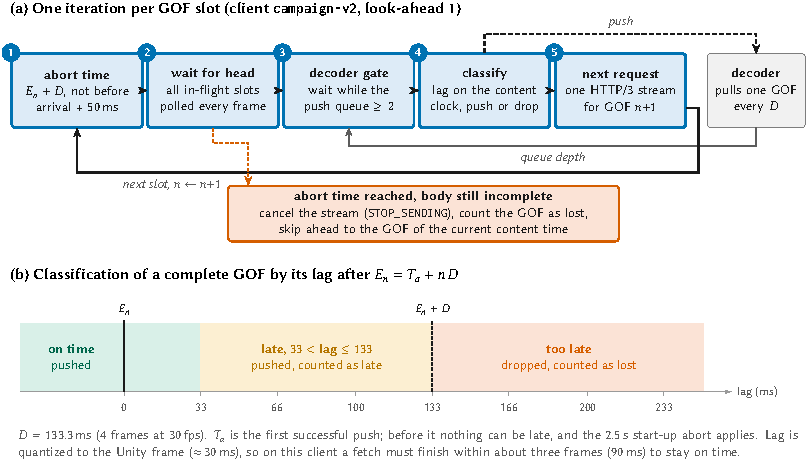
\includegraphics[width=\textwidth]{figures/contrib/fig5_deadline_scheduler.pdf}
  \caption{Client playout scheduler. (a) One loop iteration per GOF slot. (b) A complete GOF is classified by its lag after its slot start on the content clock.}
  \Description{Panel a: five steps in a loop, abort time, wait for head, decoder gate, classify, next request, with a decoder pulling one GOF every 133 ms and a timeout branch that cancels the stream and skips ahead. Panel b: a lag axis with an on-time zone up to 33 ms, a late but pushed zone up to 133 ms, and a dropped zone beyond.}
  \label{fig:contrib-scheduler}
\end{figure}

\begin{figure}[t]
  \centering
  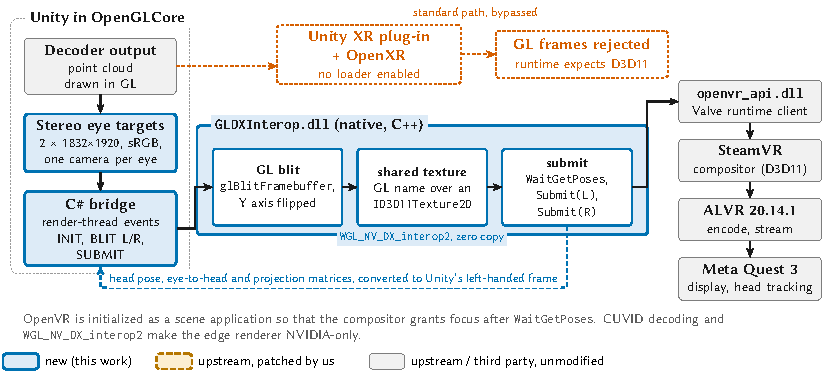
\includegraphics[width=\textwidth]{figures/contrib/fig6_gldx_openxr_bypass.pdf}
  \caption{GLDXInterop bypasses Unity's XR plug-in and OpenXR. Eye textures are copied on the GPU into D3D11 textures shared through \texttt{WGL\_NV\_DX\_interop2} and submitted to OpenVR directly.}
  \Description{The decoder output is rendered into two eye targets. A C\# bridge triggers render-thread events in the native plugin, which blits each eye into a shared texture and submits it to OpenVR, then SteamVR, ALVR and the Quest 3. A dashed red path shows the standard OpenXR route, where GL frames are rejected. A dashed blue path returns head pose and projection matrices to Unity.}
  \label{fig:contrib-gldx}
\end{figure}

\begin{figure}[t]
  \centering
  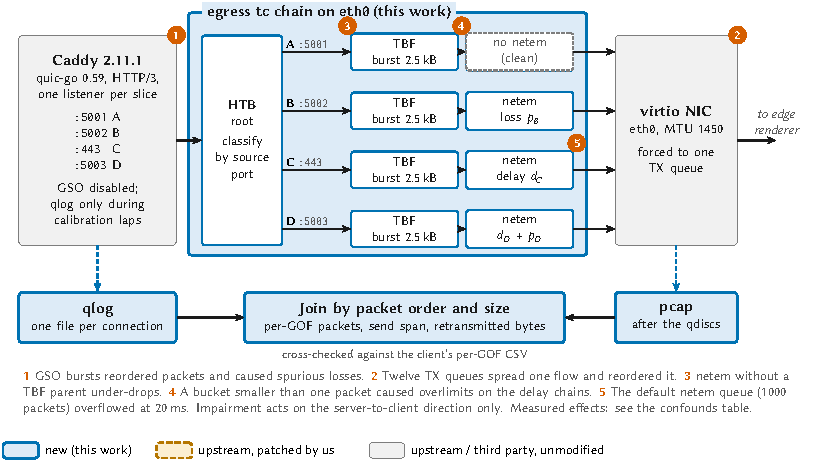
\includegraphics[width=\textwidth]{figures/contrib/fig7_origin_impairment.pdf}
  \caption{Origin, impairment chain and server-side measurement. Numbered badges locate the transport confounds of Table~\ref{tab:confounds}.}
  \Description{Caddy with four listeners feeds an HTB root that classifies by source port into four chains of TBF and netem, for clean, loss, delay and combined slices, then a virtio NIC with one transmit queue. qlog from Caddy and pcap after the qdiscs are joined into per-GOF metrics.}
  \label{fig:contrib-origin}
\end{figure}

\begin{figure}[t]
  \centering
  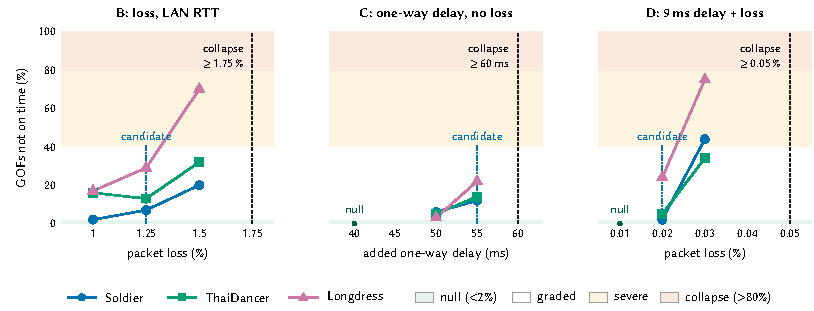
\includegraphics[width=\textwidth]{figures/contrib/fig8_transport_map.pdf}
  \caption{Transport map of the campaign client measured with the headless harness: mean fraction of GOFs not on time per rung. Only graded and severe rungs are plotted per sequence; null rungs stay below 2\% for every sequence. Loss below 1\% at LAN RTT was null.}
  \Description{Three line charts. Loss only at LAN RTT: graded from 1 to 1.5 percent, collapse from 1.75 percent. Delay only: null at 40 ms, graded at 50 and 55 ms, collapse from 60 ms. 9 ms delay plus loss: null at 0.01 percent, graded at 0.02, severe at 0.03, collapse from 0.05 percent. Longdress is the least tolerant sequence on loss.}
  \label{fig:contrib-transport-map}
\end{figure}

\input{figures/contrib/tab_contributions}
\input{figures/contrib/tab_transport_confounds}
